\subsection{Red de Galerías Pacífico}
En este caso la captura se llevó a cabo en una red no controlada, en Galerías Pacífico, durante aproximadamente 10 minutos.
Debido a que la red no está controlada por nosotros, no sabemos la naturaleza de los equipos que intercambian inforación en la misma, pero conjeturamos que la mayoría son celulares. Este ~\ref{fig:galerias_pacifico3_10min_network} es un grafo que muestra los distintos nodos en la red junto identificados por su dirección IP.

\begin{figure}[h!]
  \centering
   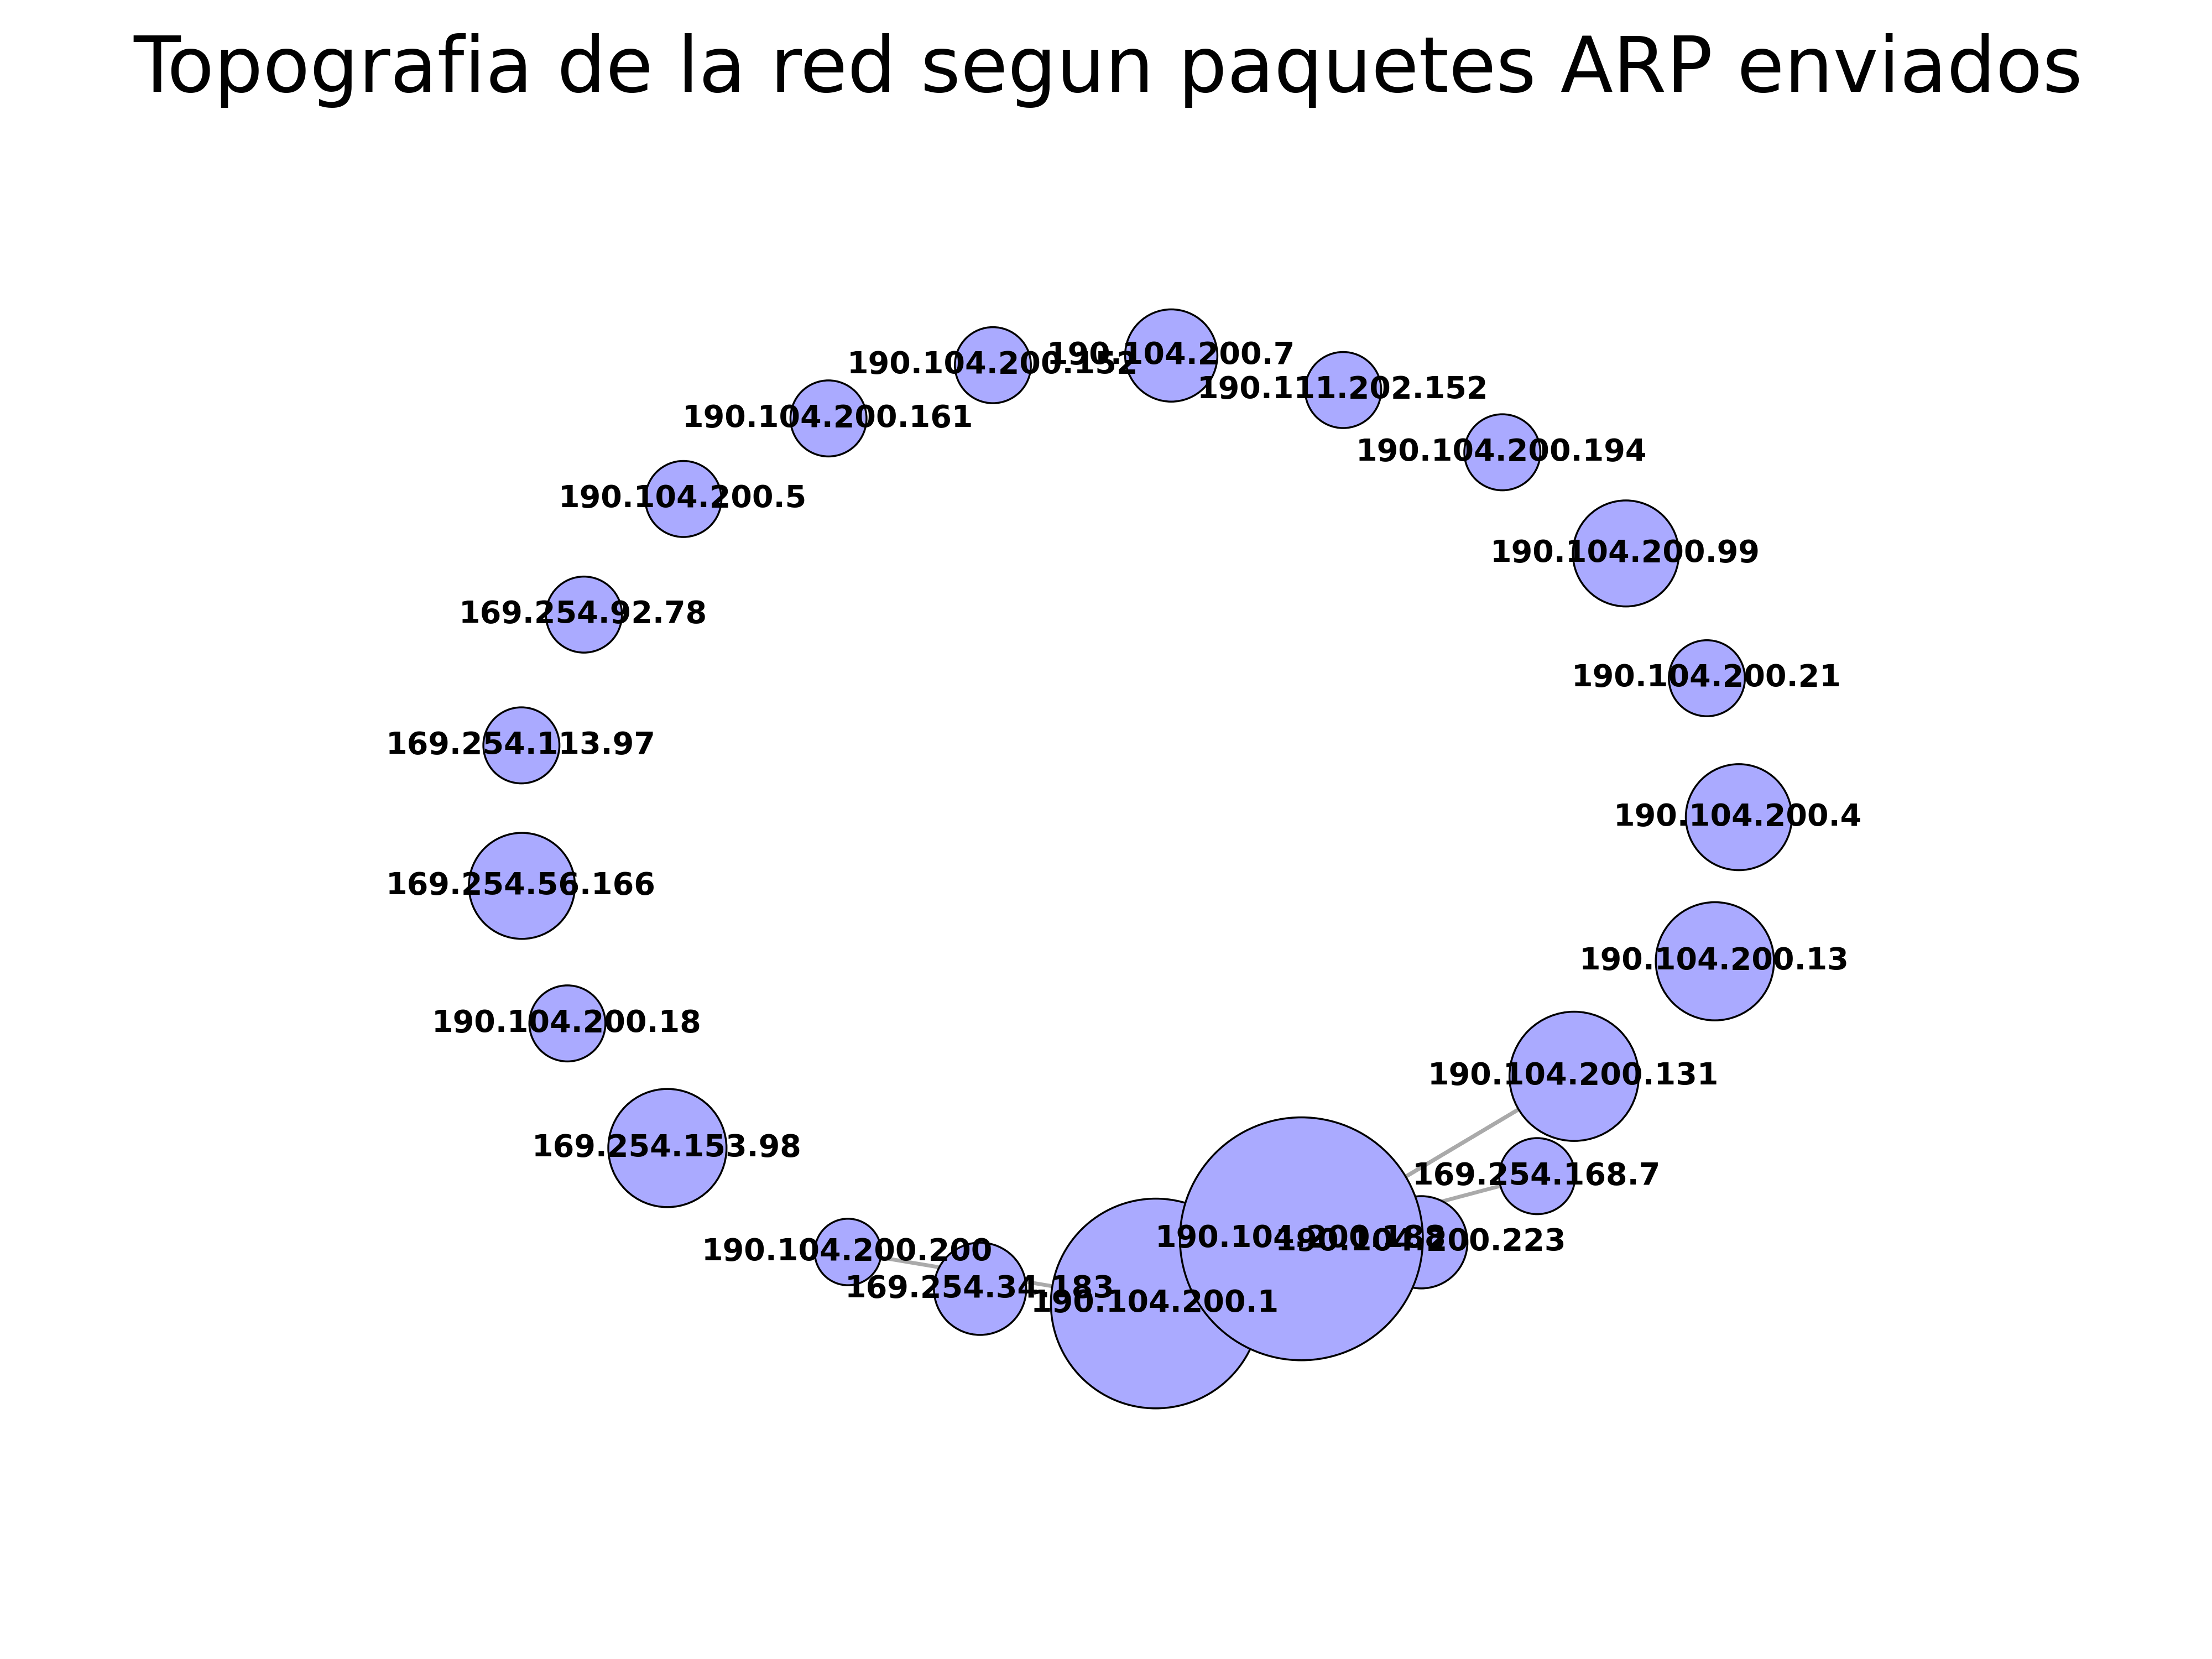
\includegraphics[width=0.7\textwidth]{graficos/galerias_pacifico3_10min_network.png}
  \caption{}
  \label{fig:galerias_pacifico3_10min_network}
\end{figure}
\FloatBarrier

\subsubsection{Paquetes capturados e información}
Mostramos ahora la frecuencia e información de cada IP en la red en ~\ref{fig:galerias_pacifico3_10min_pie_arp} y ~\ref{fig:galerias_pacifico3_10min_pie_arp_information}.


\begin{figure}[h!]
  \centering
   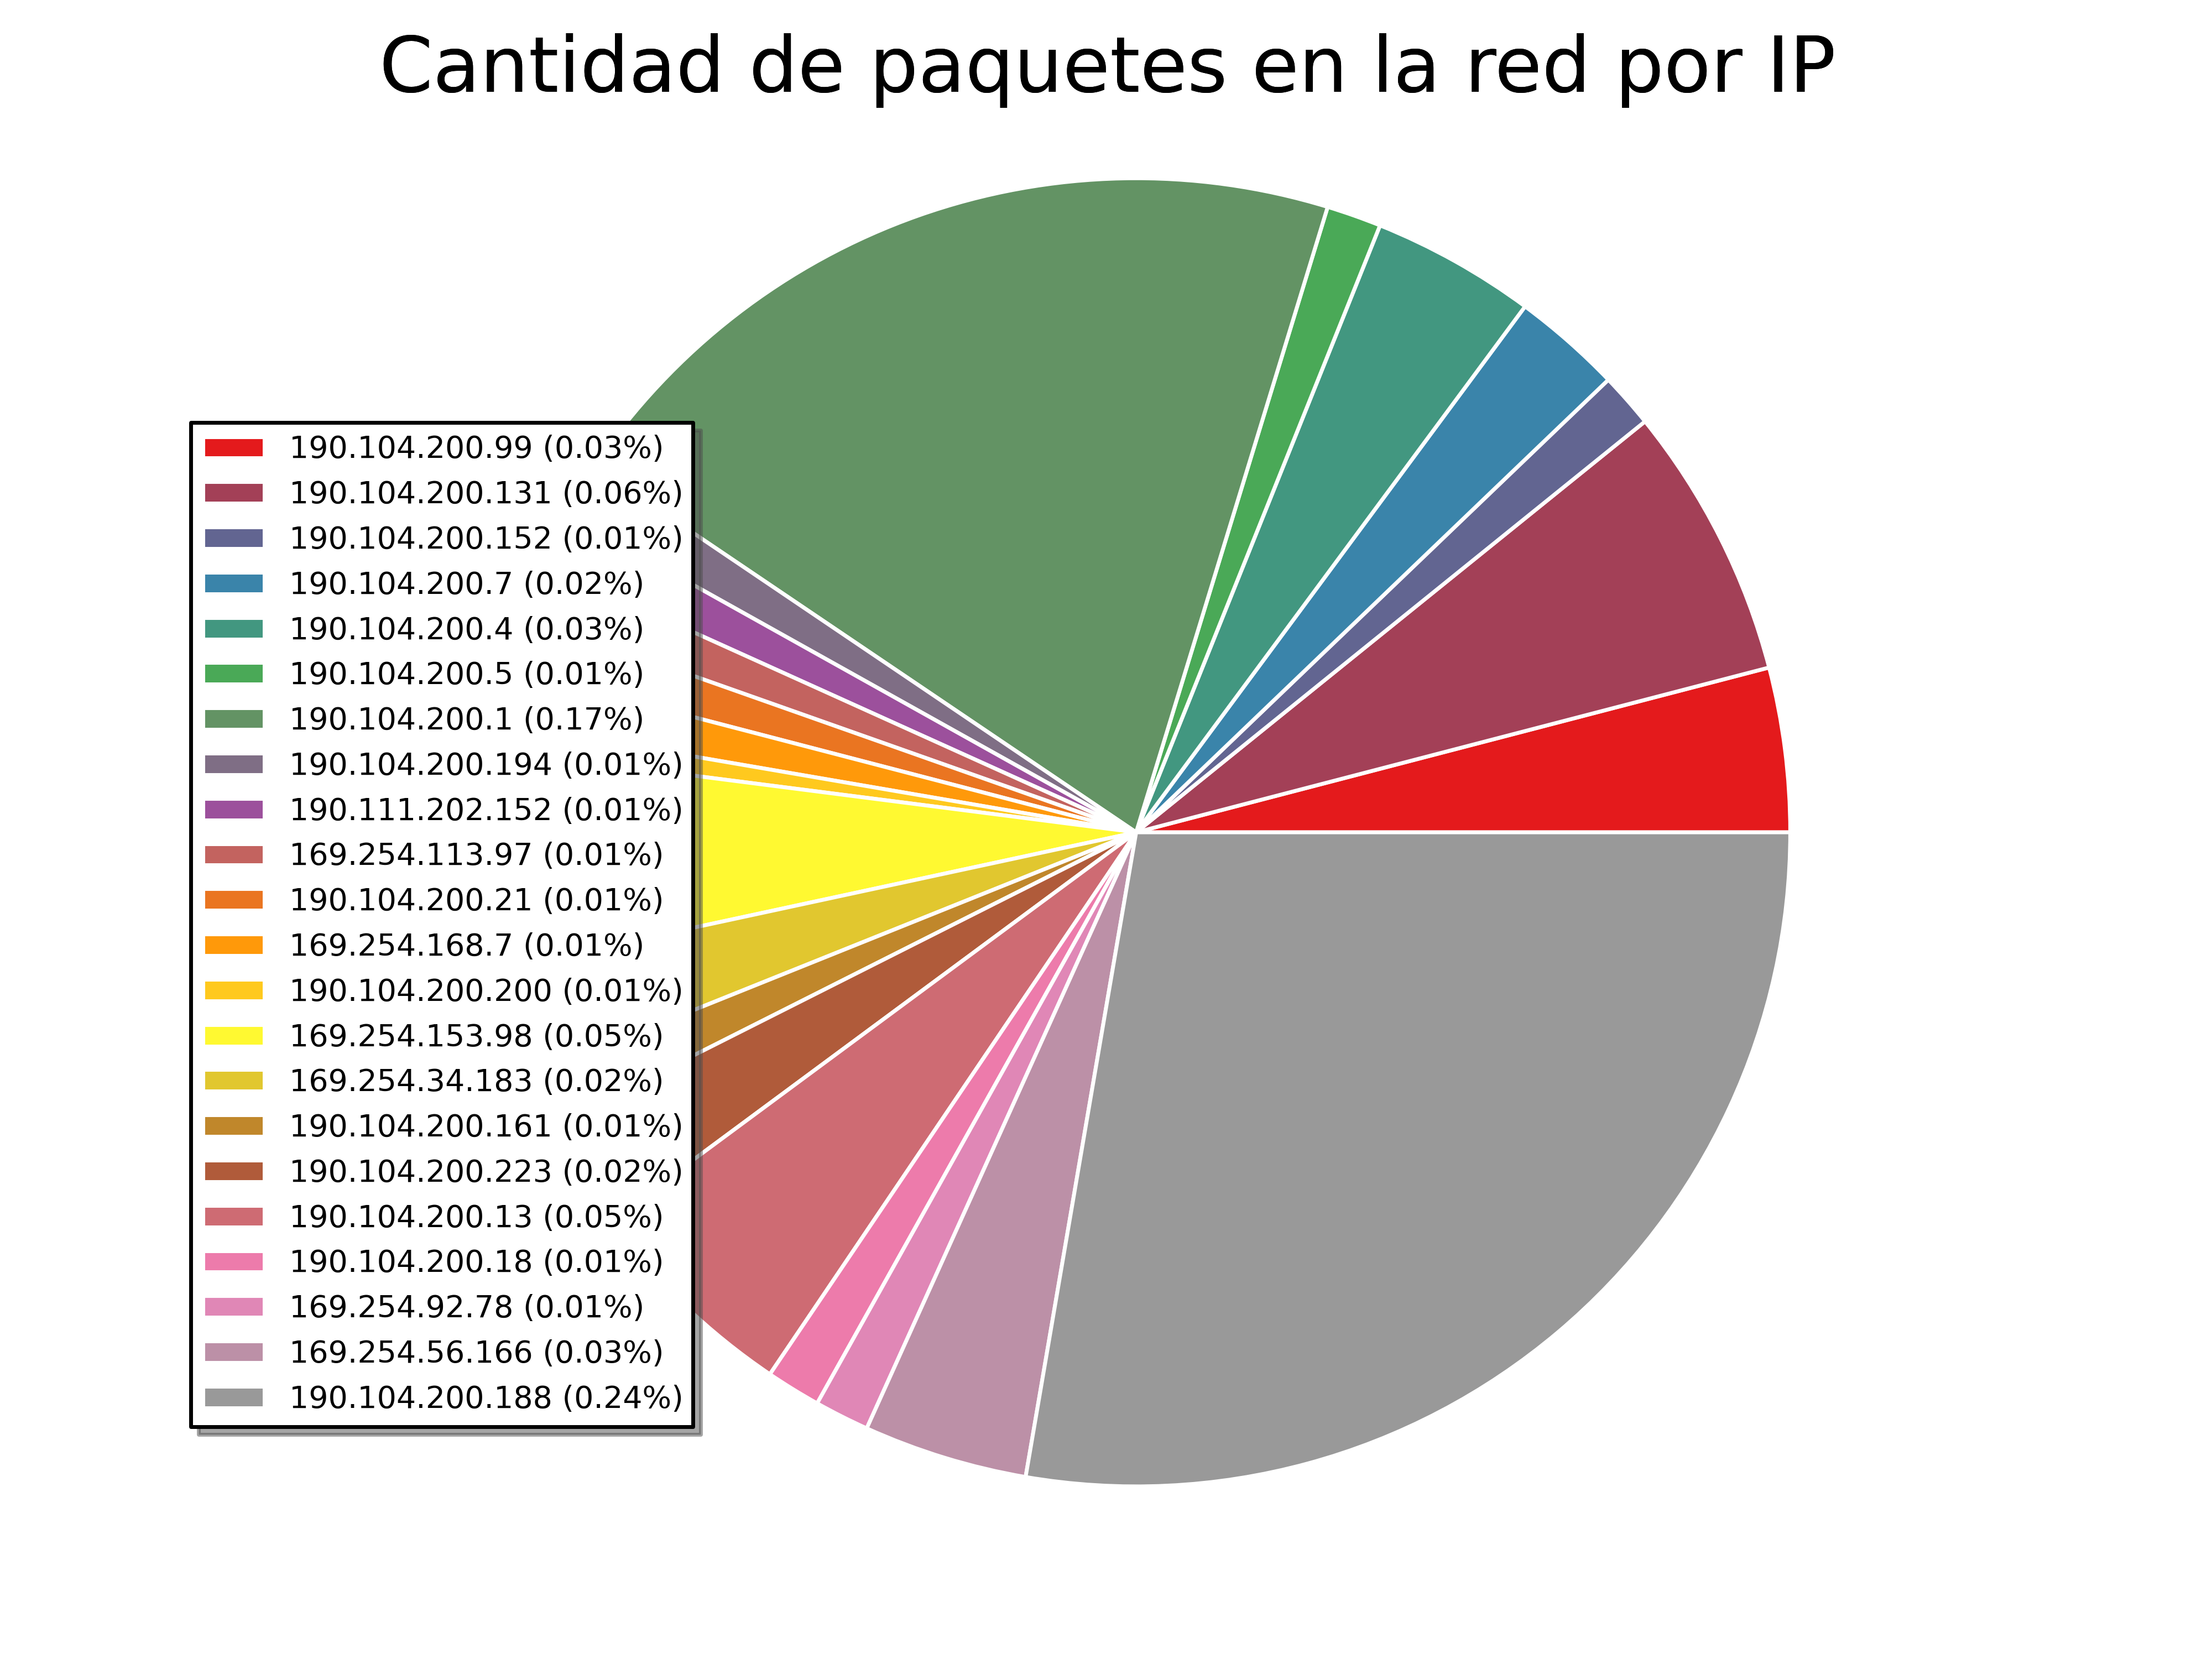
\includegraphics[width=0.7\textwidth]{graficos/galerias_pacifico3_10min_pie_arp.png}
  \caption{}
  \label{fig:galerias_pacifico3_10min_pie_arp}
\end{figure}

\begin{figure}[h!]
  \centering
   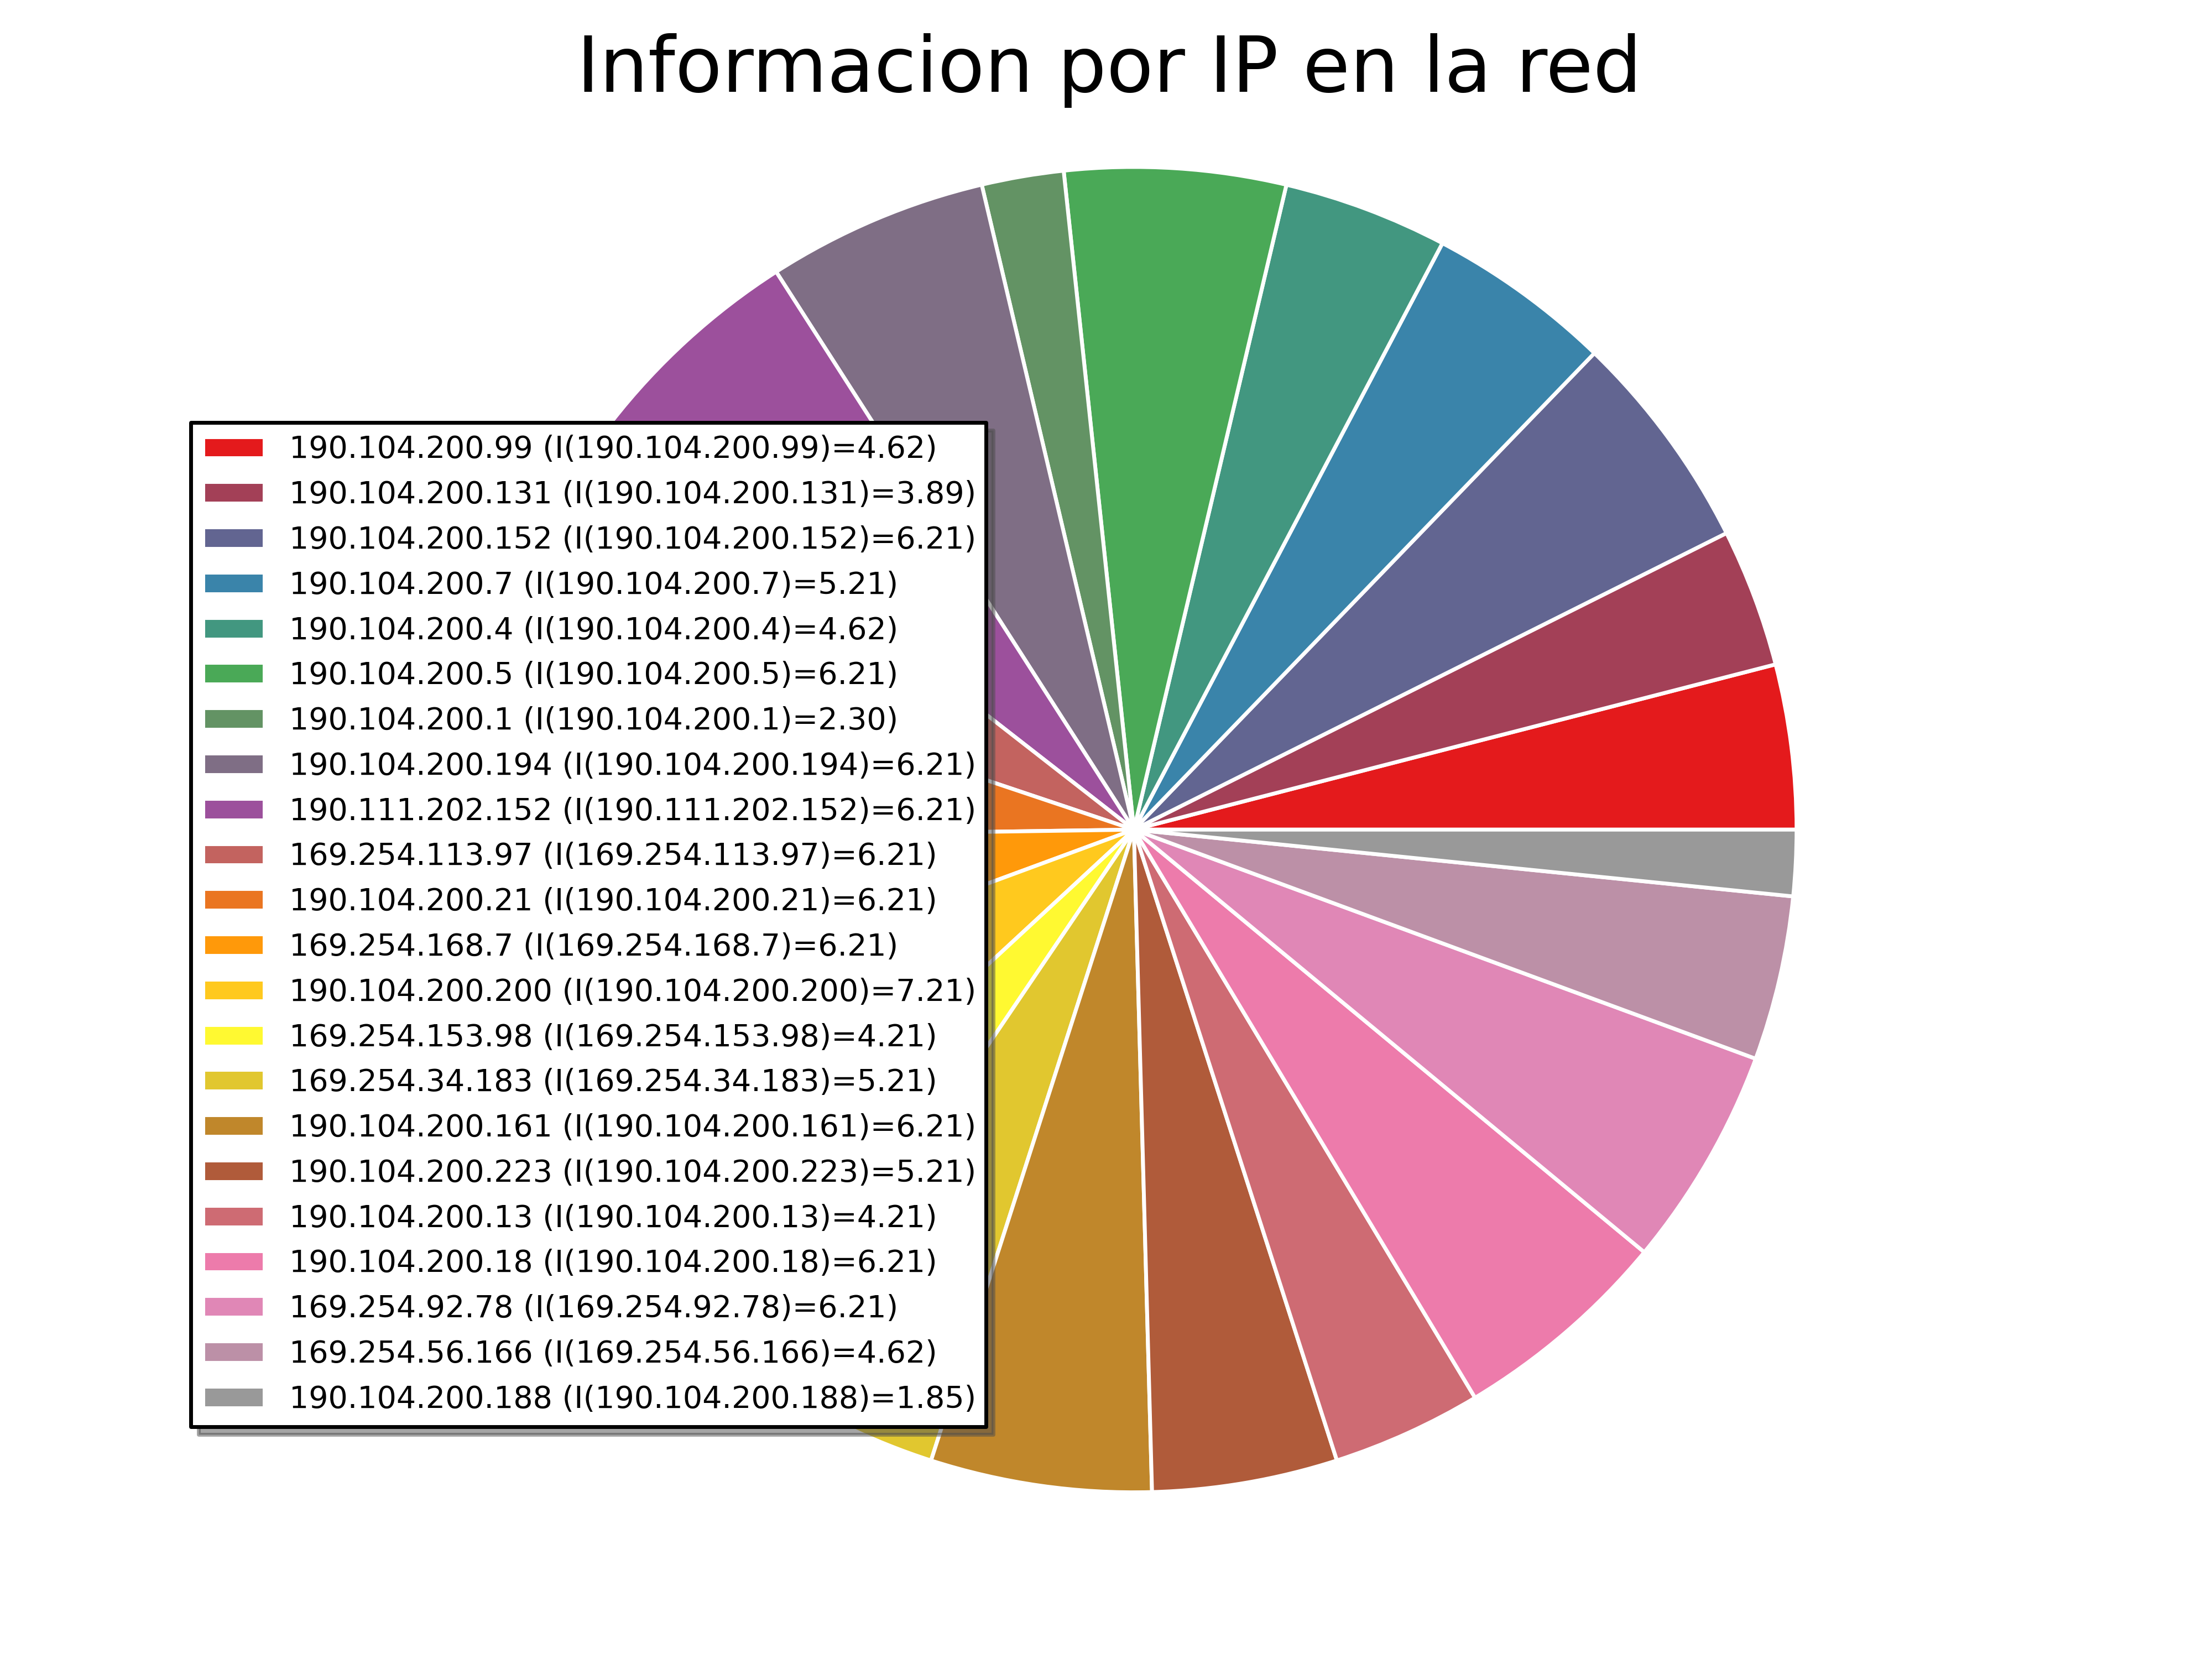
\includegraphics[width=0.7\textwidth]{graficos/galerias_pacifico3_10min_pie_arp_information.png}
  \caption{}
  \label{fig:galerias_pacifico3_10min_pie_arp_information}
\end{figure}

Podemos ver que las IP's distinguidas son 192.104.200.5, 190.104.200.1 y 190.104.200.188. 
\\

Los resultados del experimento para determinar protocolos importantes se resumen en los gráficos ~\ref{fig:galerias_pacifico3_10min_pie_type} y ~\ref{fig:galerias_pacifico3_10min_pie_type_information}. Se puede notar que el protocolo IPV4 es el más frecuente (y por ende el que brinda enos información).

\begin{figure}[h!]
  \centering
   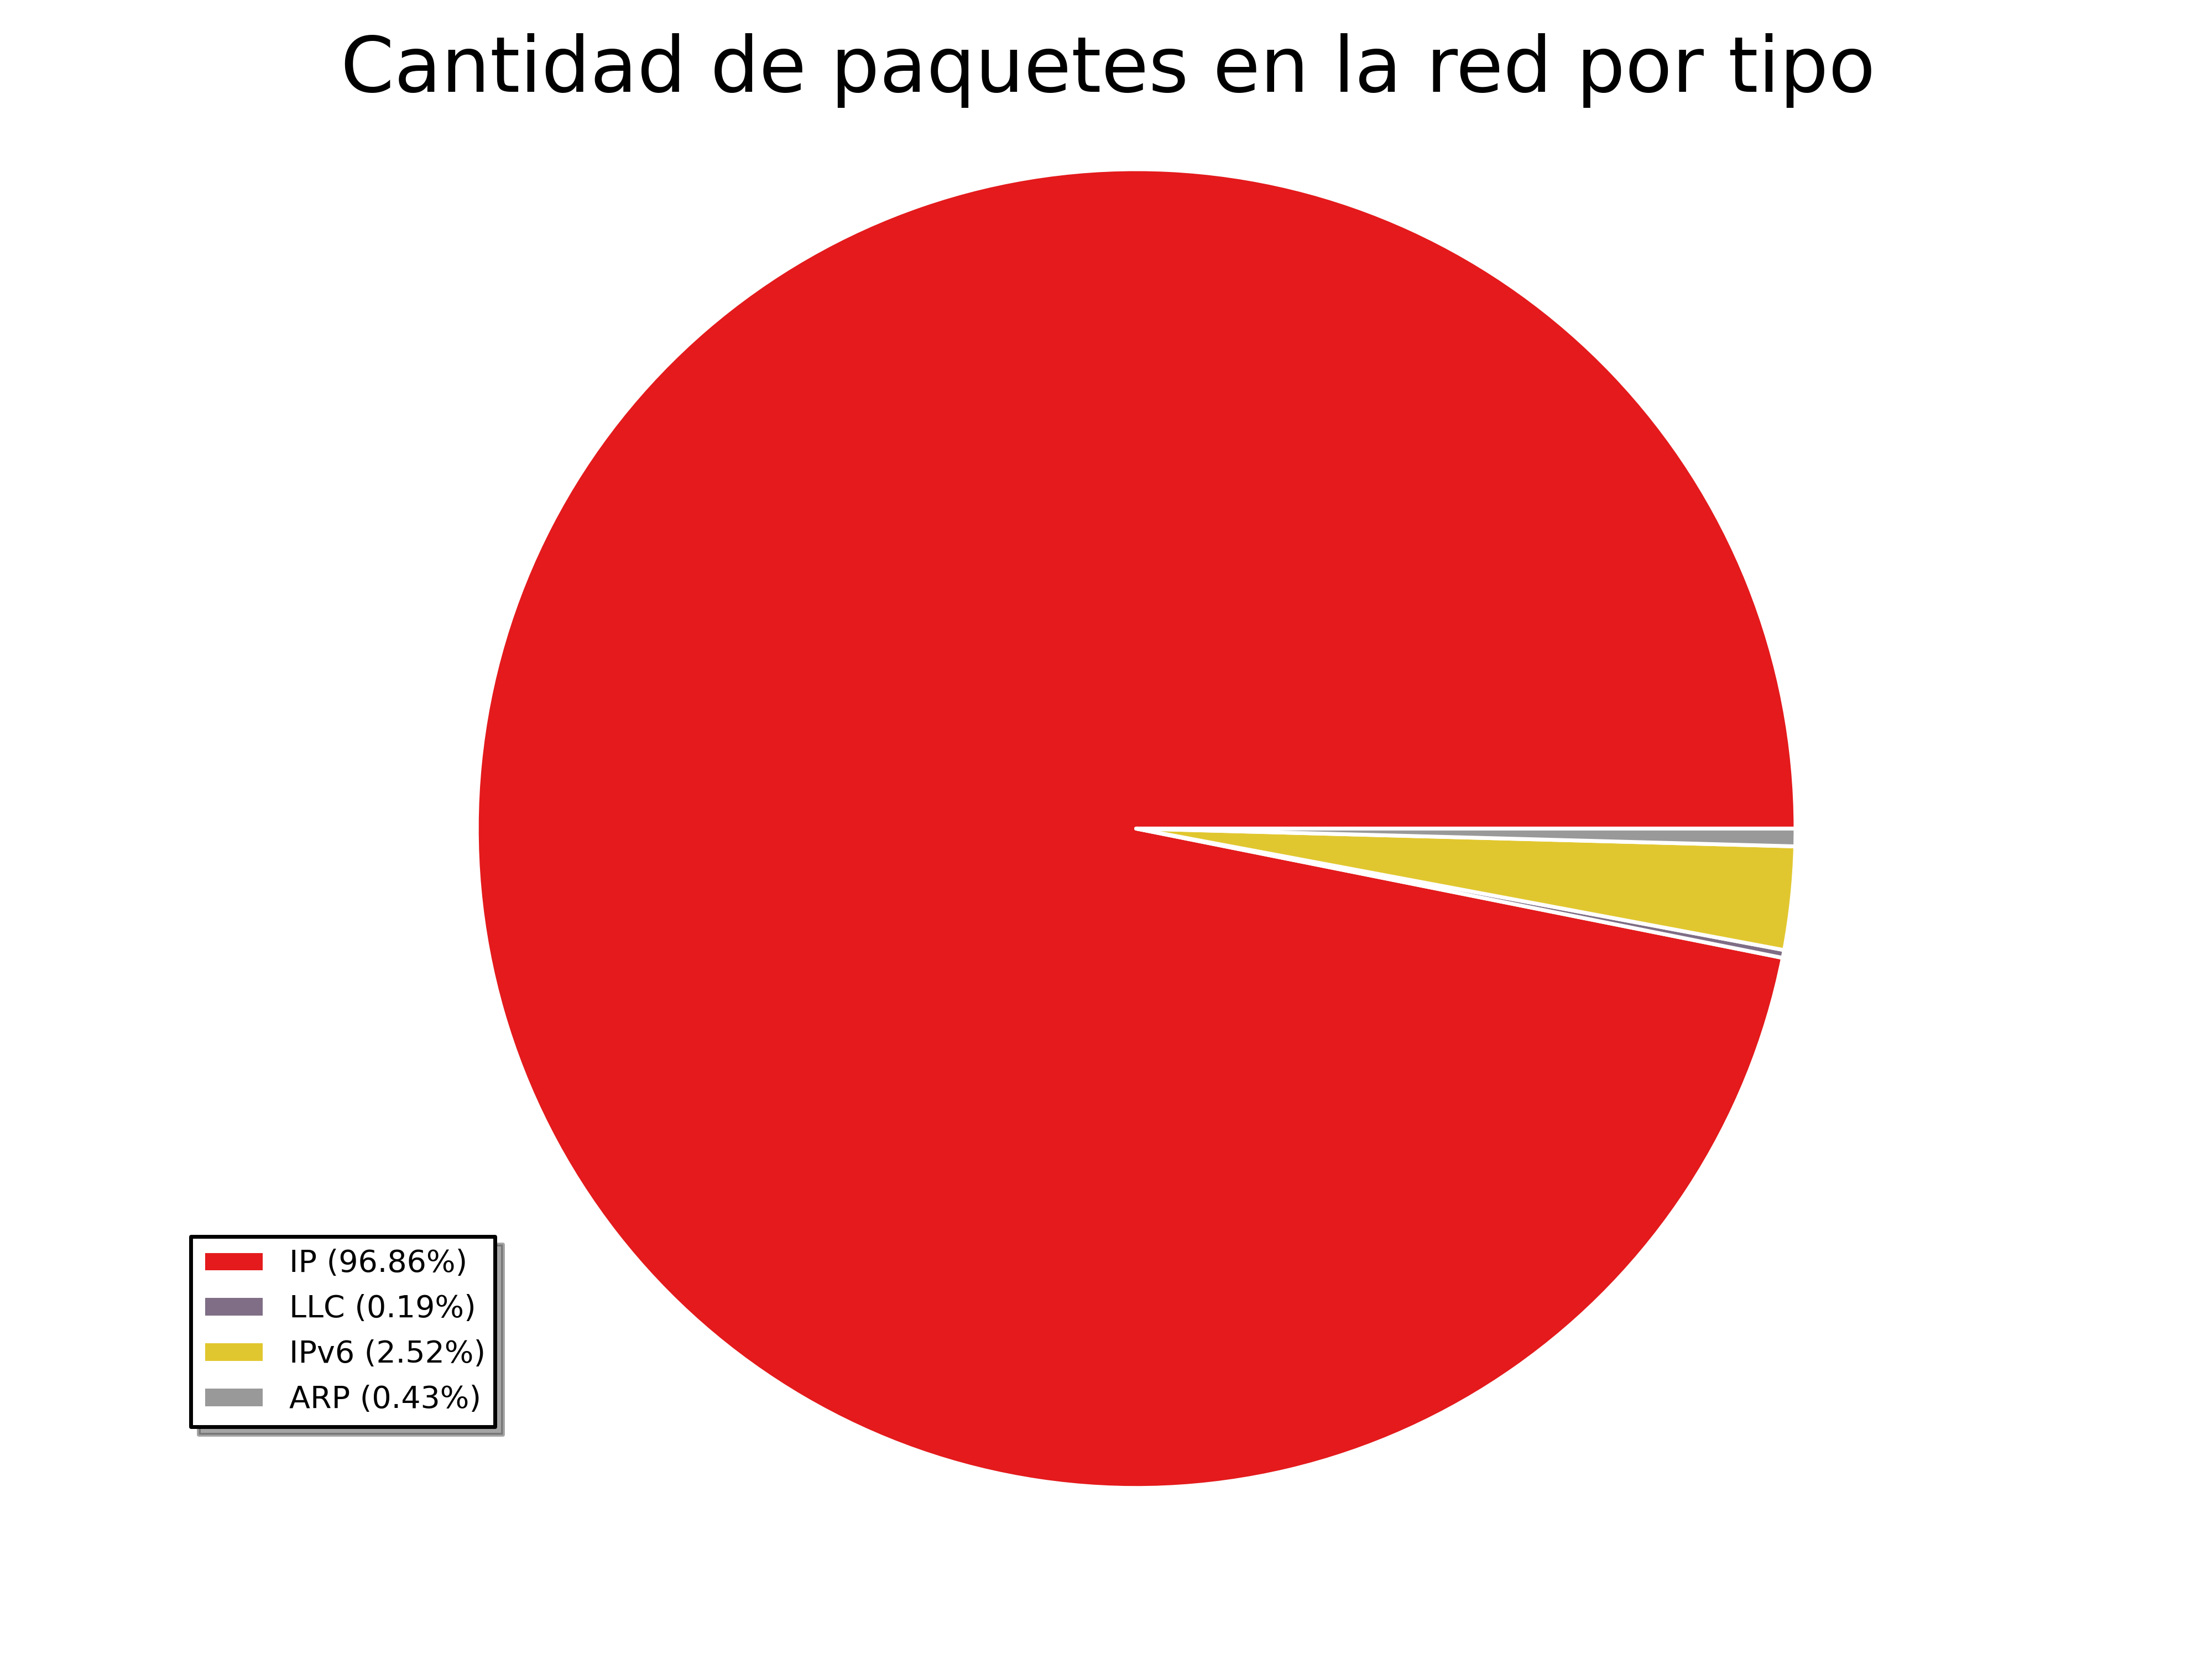
\includegraphics[width=0.7\textwidth]{graficos/galerias_pacifico3_10min_pie_type.png}
  \caption{}
  \label{fig:galerias_pacifico3_10min_pie_type}
\end{figure}

\begin{figure}[h!]
  \centering
   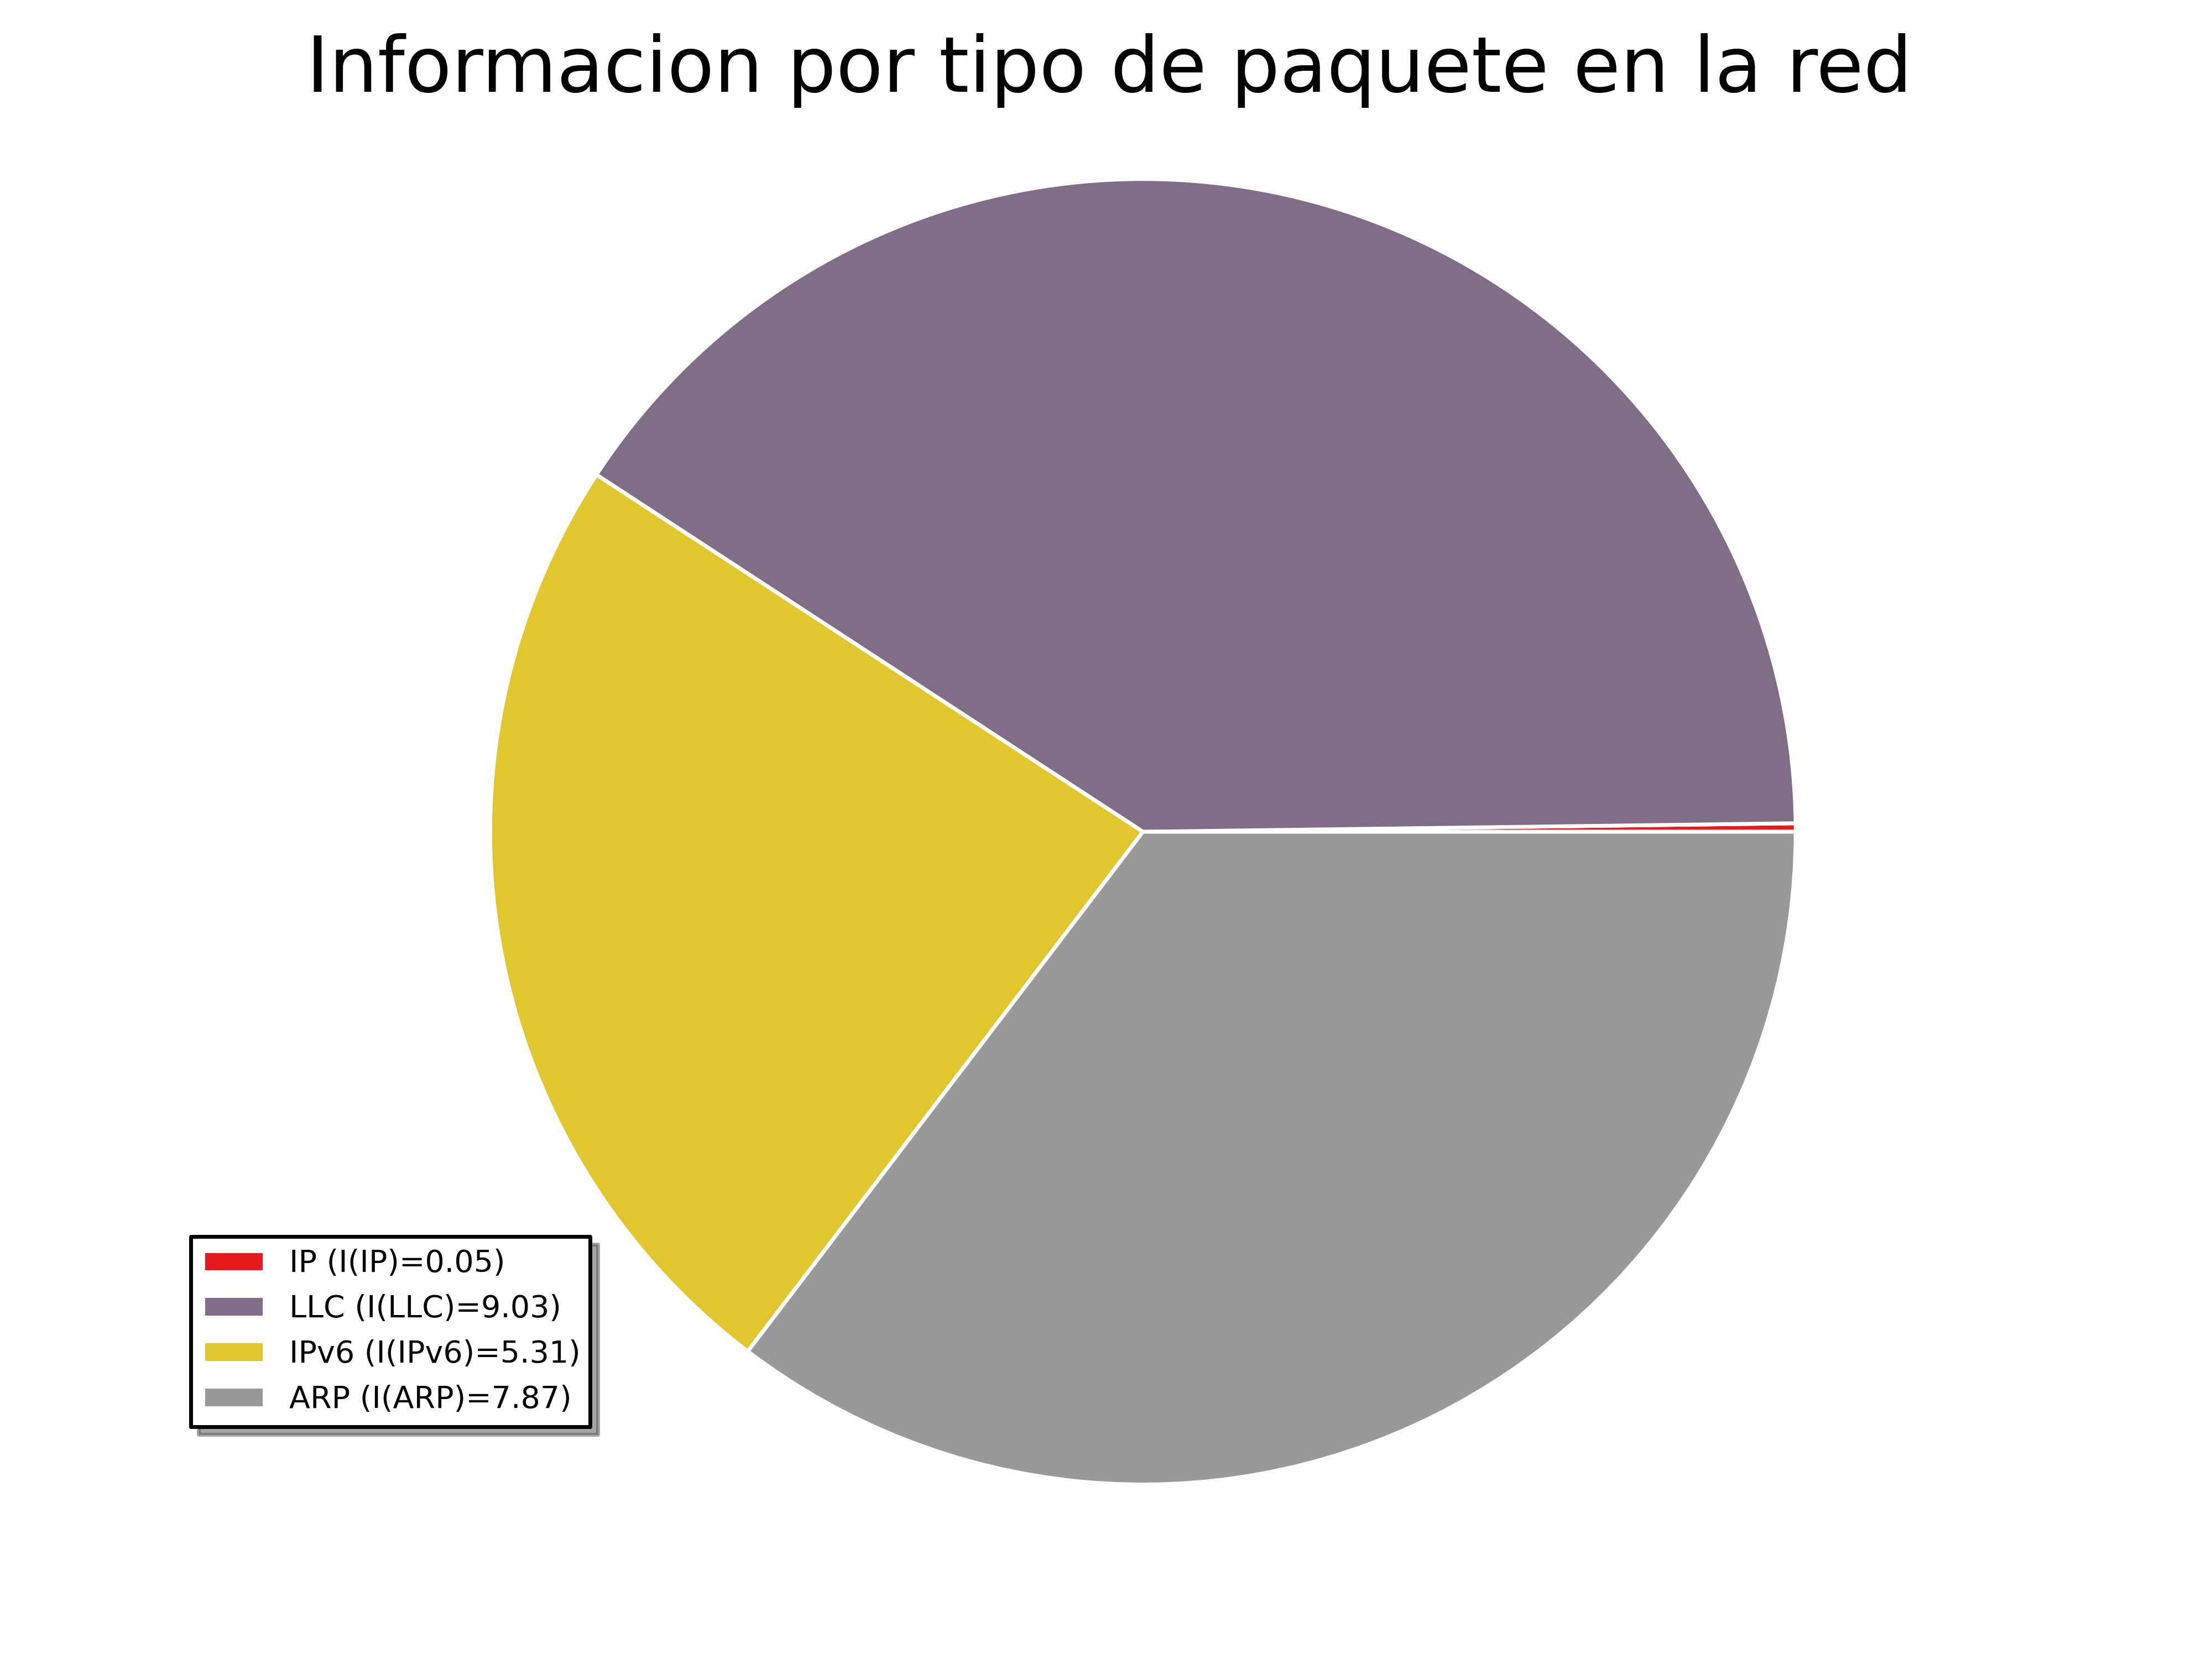
\includegraphics[width=0.7\textwidth]{graficos/galerias_pacifico3_10min_pie_type_information.png}
  \caption{}
  \label{fig:galerias_pacifico3_10min_pie_type_information}
\end{figure}

\subsubsection{Histogramas (de IPs y protocolos)}
En esta sección usamos el consepto de entropía para deducir características de la red analizada. Al igual que en las otras redes, podemos ver en ~\ref{fig:galerias_pacifico3_10min_hist_type} y en ~\ref{fig:galerias_pacifico3_10min_hist_arp} que la entropía en la fuente $S$ es menor que en la fuente $S_1$, debido a que en la primera, el protocolo IPV4 es mucho más frecuente que los demás.


\begin{figure}[h!]
  \centering
   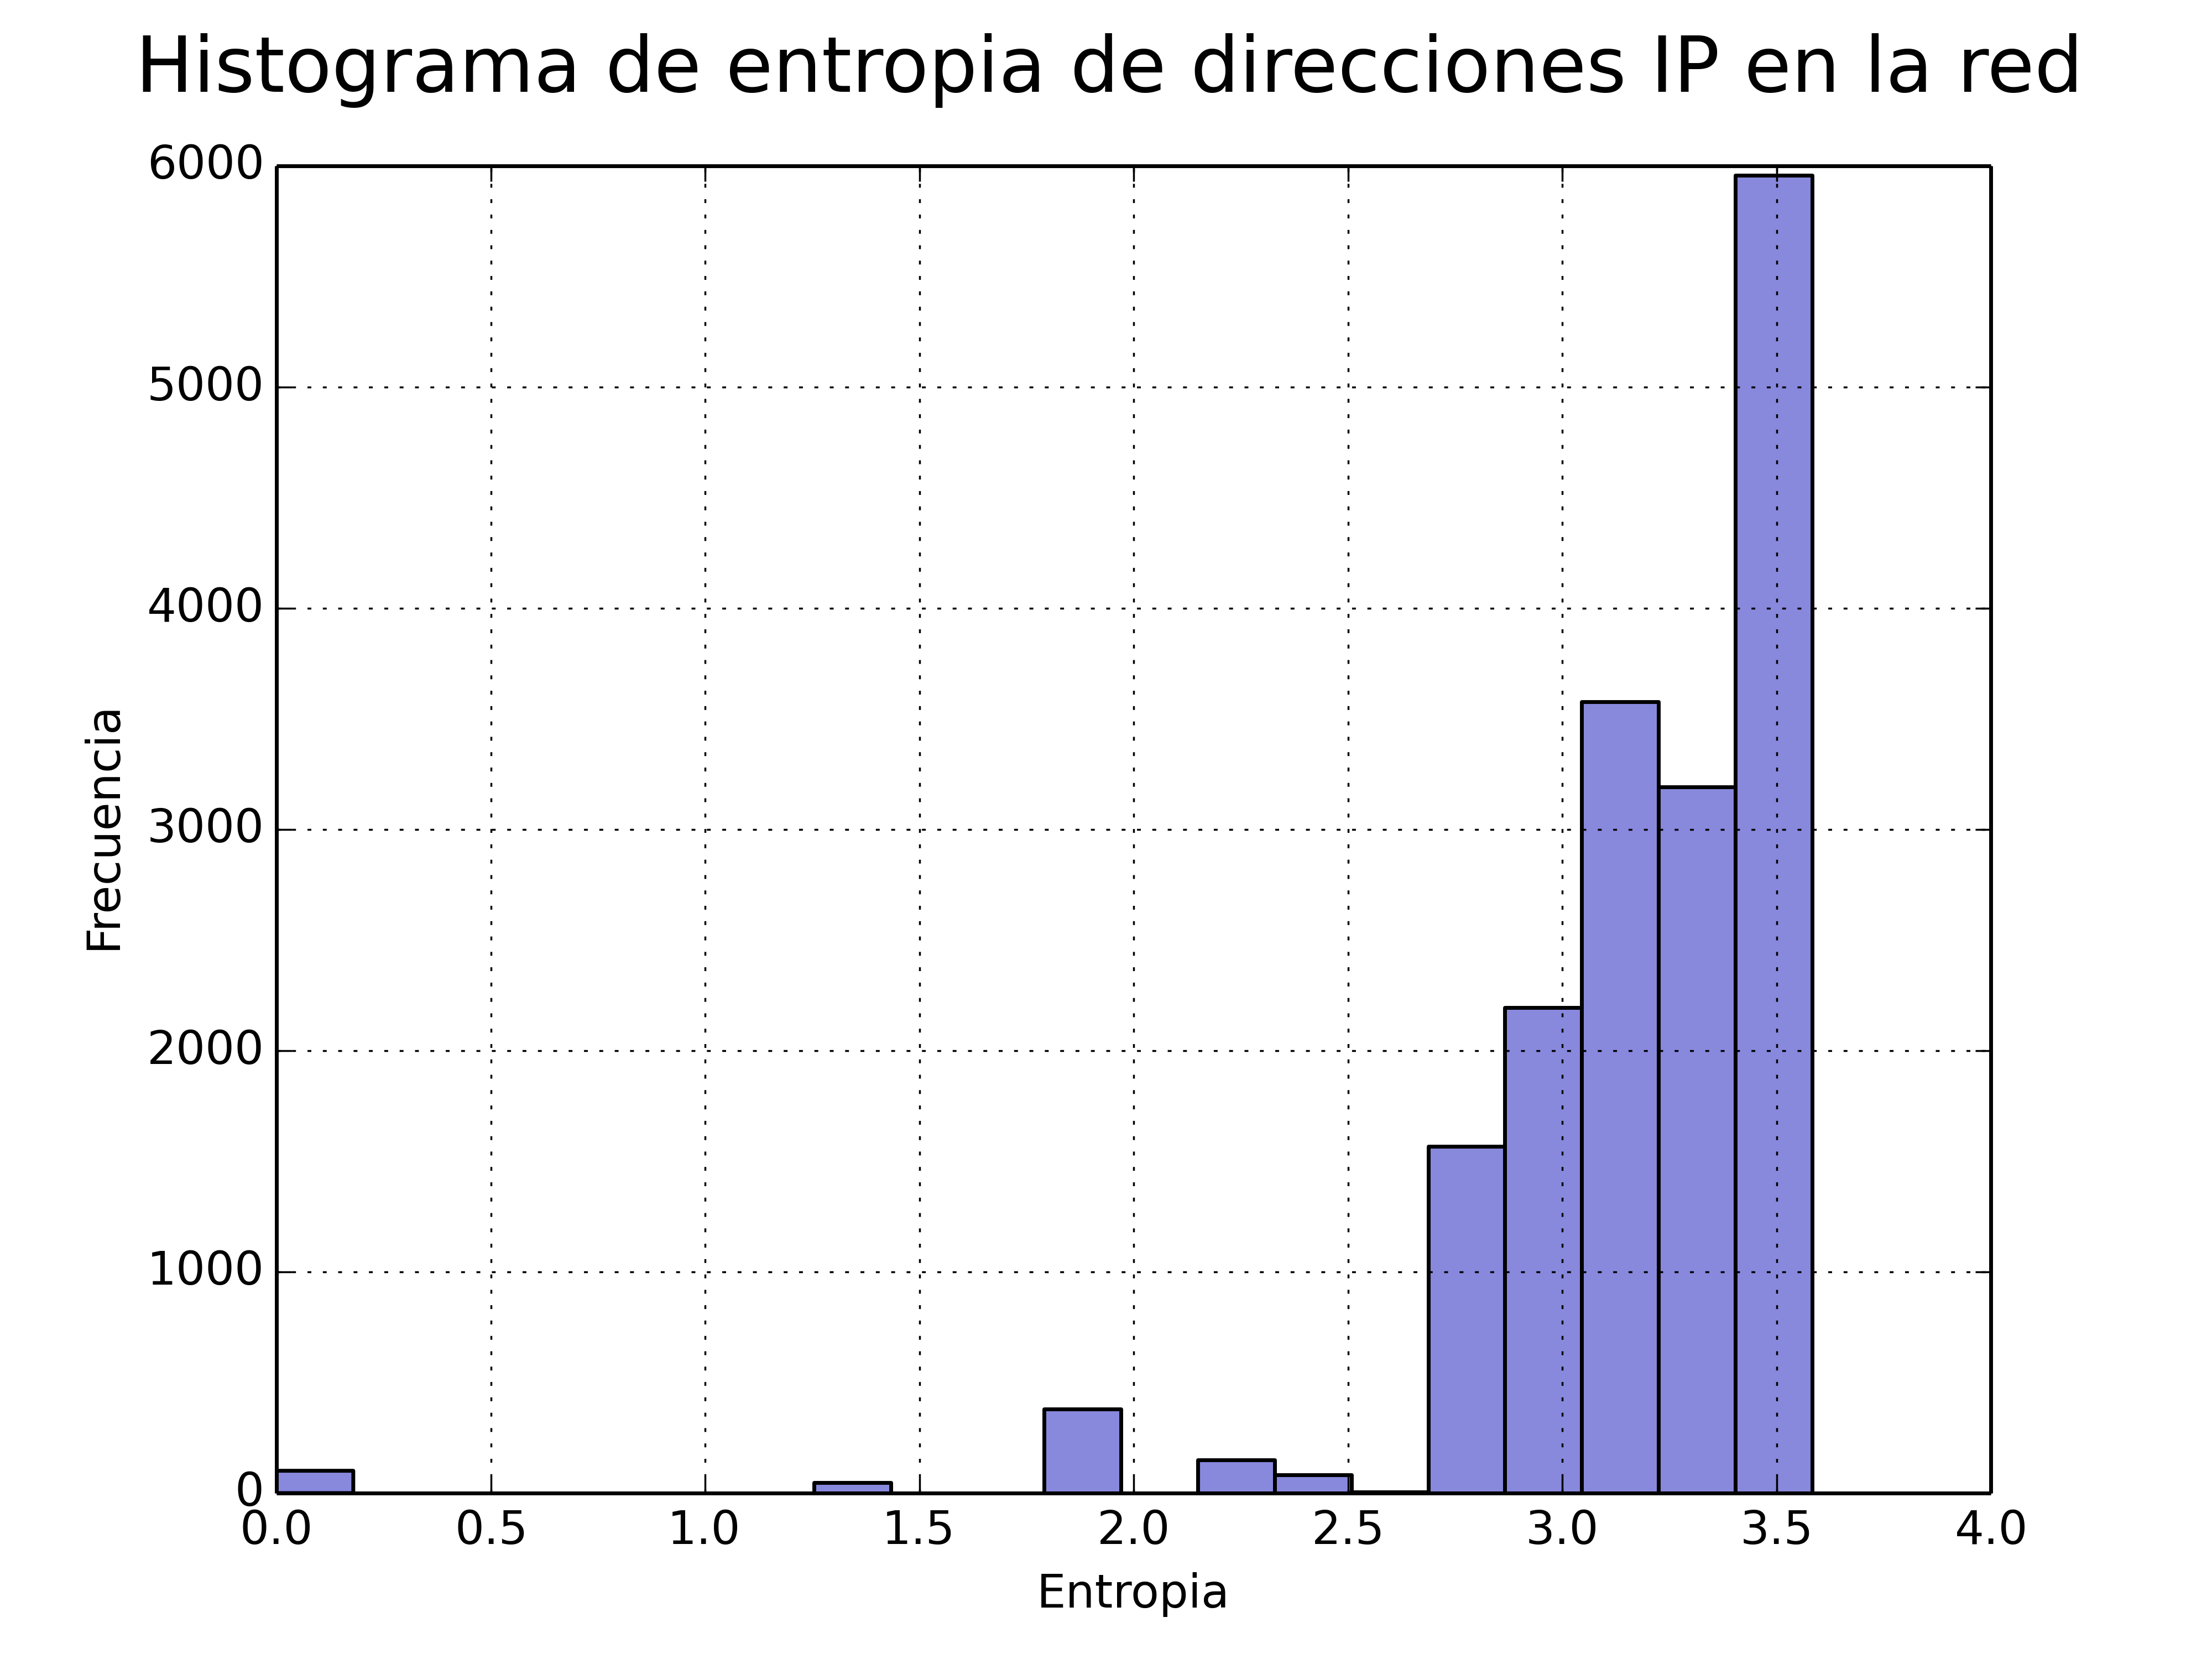
\includegraphics[width=0.7\textwidth]{graficos/galerias_pacifico3_10min_hist_arp.png}
  \caption{}
  \label{fig:galerias_pacifico3_10min_hist_arp}
\end{figure}

\begin{figure}[h!]
  \centering
   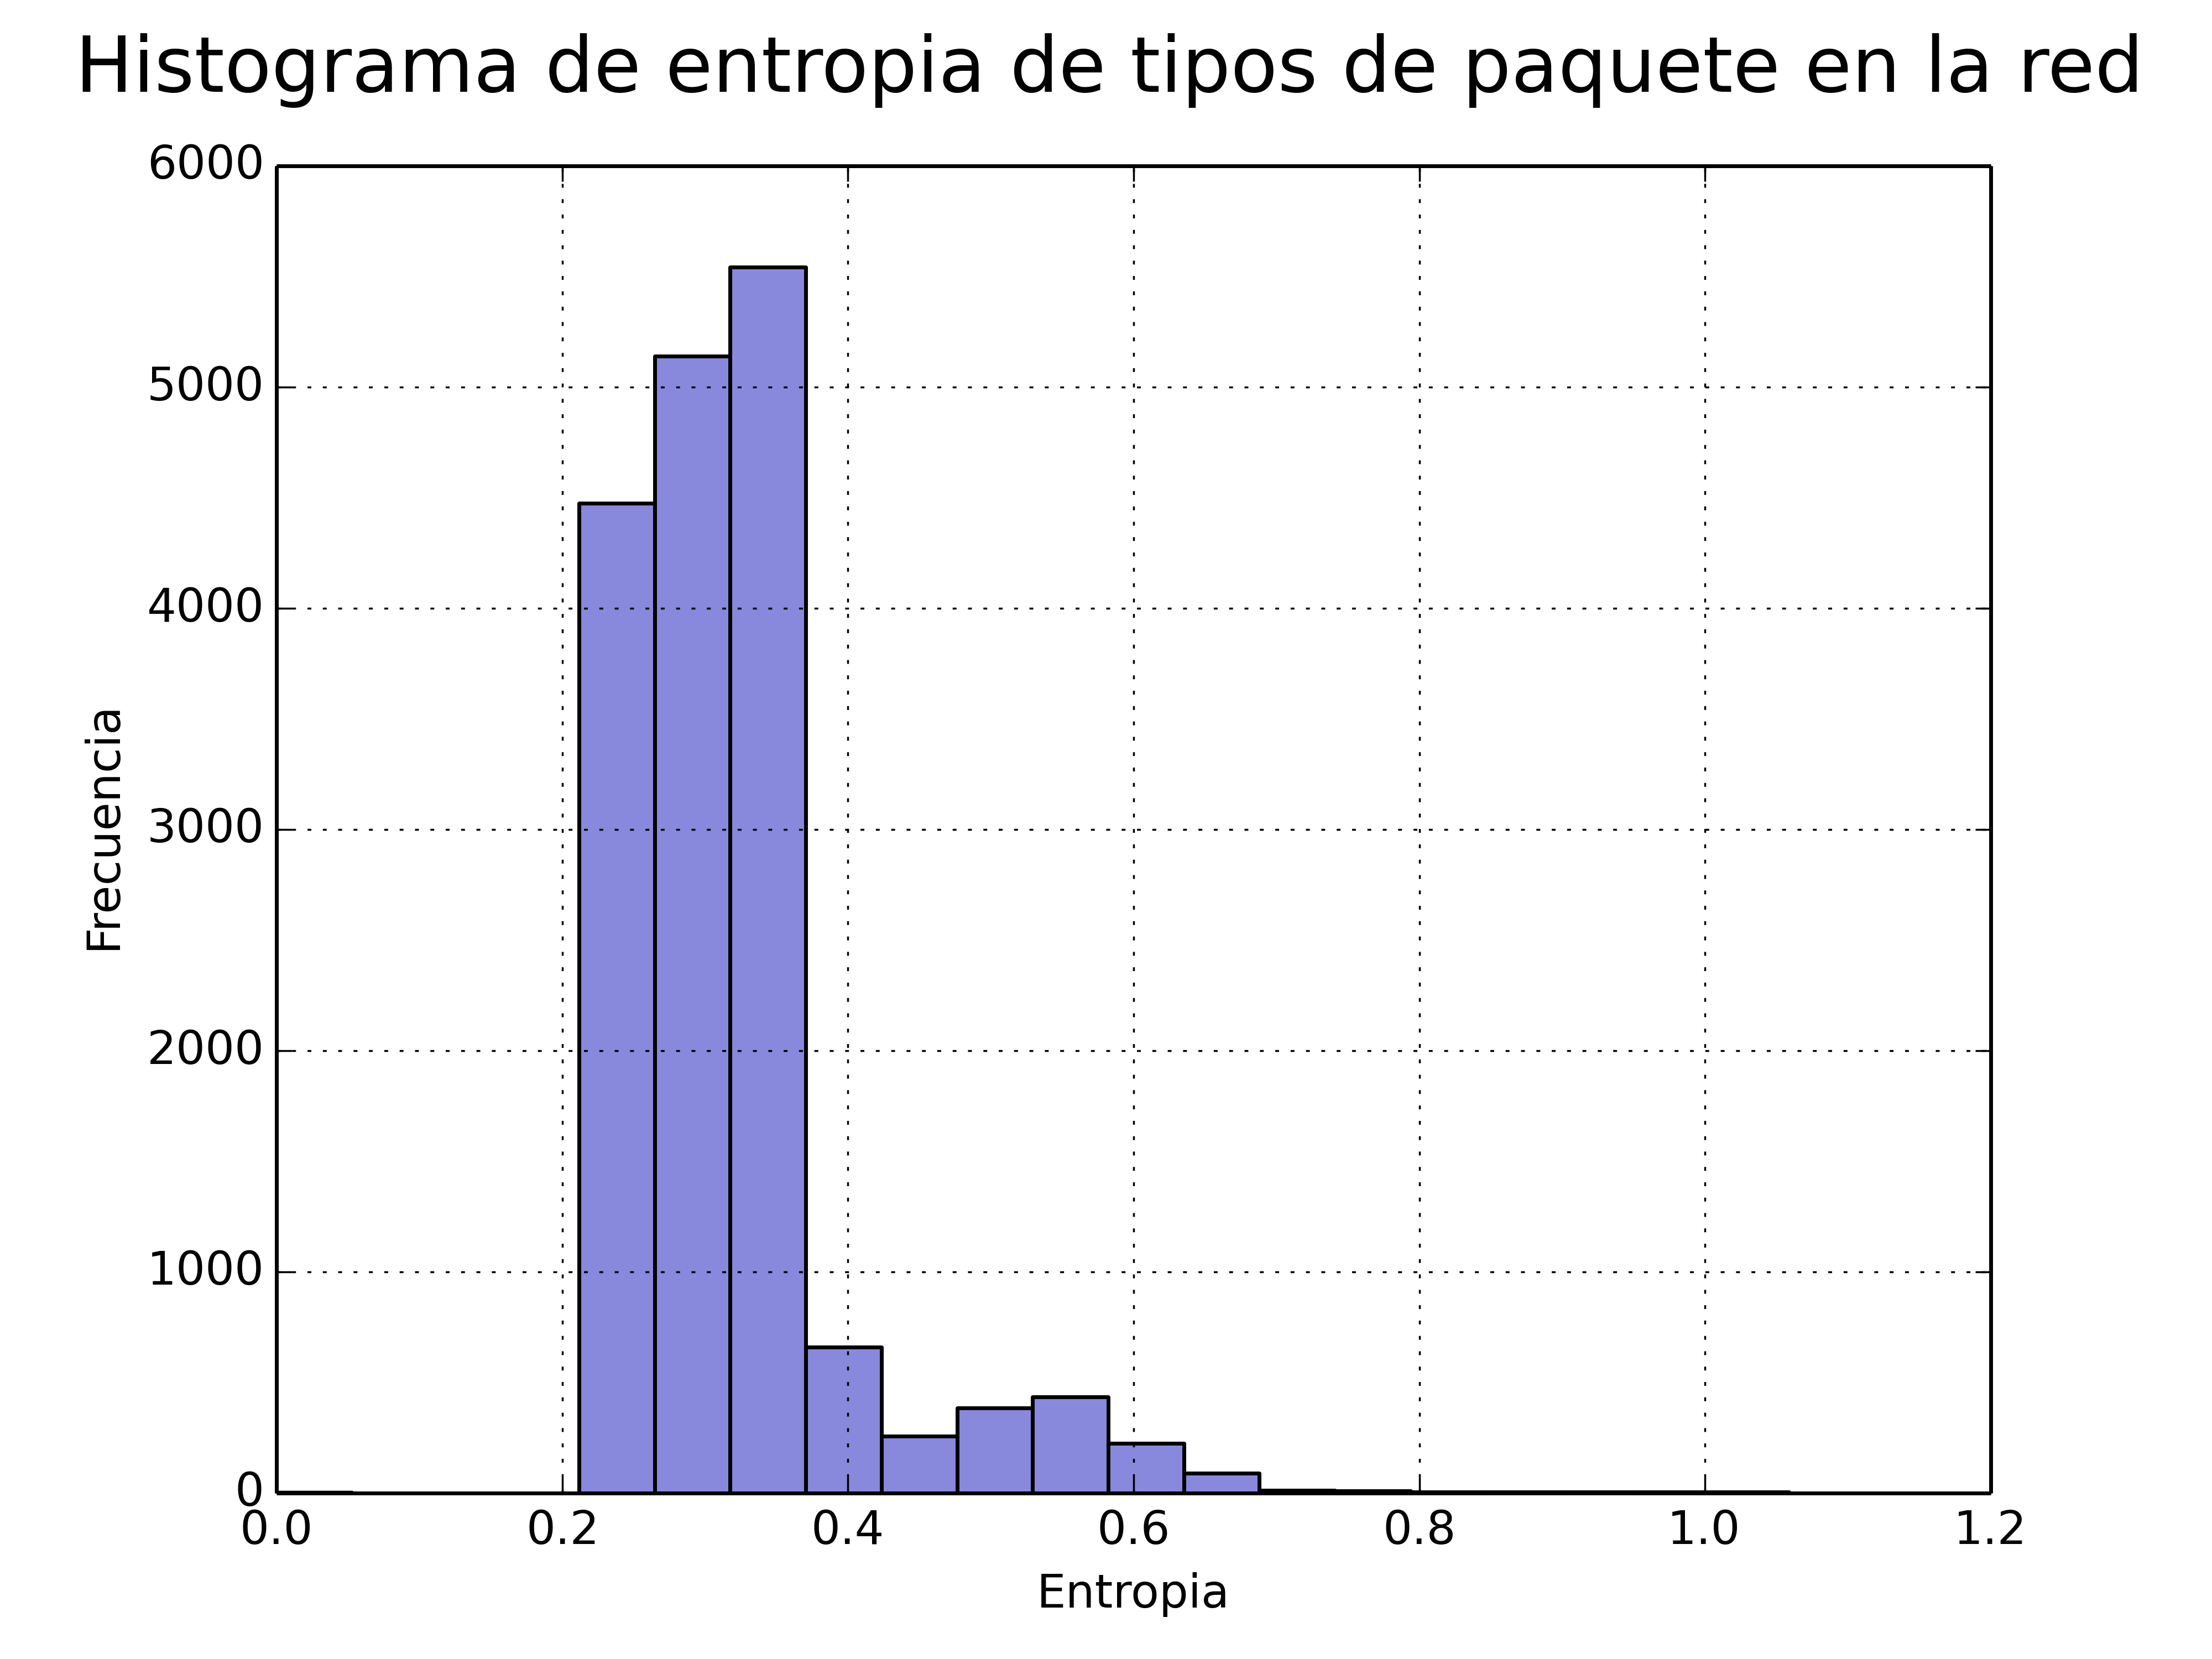
\includegraphics[width=0.7\textwidth]{graficos/galerias_pacifico3_10min_hist_type.png}
  \caption{}
  \label{fig:galerias_pacifico3_10min_hist_type}
\end{figure}




